\chapter{Logic and Objects}
\label{lo}
\index{Logic and Objects}
\lettrine[nindent=0.1em]{T}{he fundamental concept} behind \go's object notation is the \emph{labeled theory}. A theory is simply a set of facts that is known about some concept. Of course, \go theories are about more than predicates: functions, action procedures and grammars are also part of what can be known about a concept.

A label is a term that identifies the theory. In fact, \emph{all} terms are labels of some kind of theory -- that is \go's equivalent of that famous phrase found in OO texts: everything is an object.

\begin{figure}
%\begin{boxed}
\centering
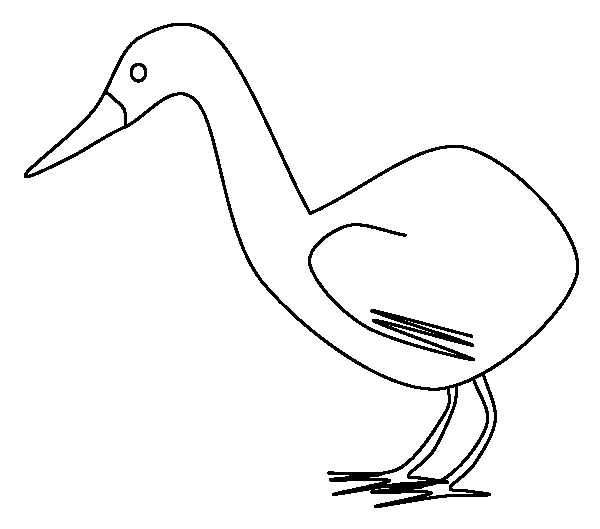
\includegraphics[width=2.5in]{bird}
%\end{boxed}
\caption{\label{lo:bird:class}One theory about \q{birdness}}
\end{figure}

The relationship between sets of facts and a label term is analogous to the standard relationship in logic between a predicate symbol and the relation denoted by that symbol. \LO extends this concept only slightly -- by permitting a symbol to denote sets of relations and by permitting this denoting symbol to be an arbitrary term. These very minor extensions do not affect the underlying logic, but make a big difference to the usability of the overall notation.

This foundation allows us to offer a view of object oriented programming that is quite close to the intuition offered in languages such as Java and Smalltalk; but in a way that is compatible with the logic under-pinnings of \go. Like Java, we have objects, classes, inheritance and even interfaces. Similarly, using the familiar dot operator to access a method of an object is equivalent to invoking the knowledge identified by a particular label.

\go's class notation is based on `Logic and Objects' \cite{fgm:92} with some simplifications and modifications to incorporate \go's type system and the notion of a stateful \emph{object} as well as a class. It provides a straightforward technique to build large scale systems and to represent knowledge. 

\section{Class notation}
\label{objects:class}
\index{class!notation}
A \go \emph{class} is defined with a combination of an optional \emph{class body} and zero or more \emph{class rules}. Class bodies give the implementation of methods and other exported values and class rules express the inheritance relationships with other classes.

\begin{program}
\vspace{0.5ex}
\begin{alltt}
birdness \impl \{ no_of_legs:[number]\{\}. mode:[symbol]\{\} \}.

bird:[]\conarrow{}birdness.
bird..\{
  no_of_legs(2).
  mode('fly').
\}.
\end{alltt}
\vspace{-2ex}
\caption{A \q{bird} class}
\label{lo:bird}
\end{program}

\subsection{Class types}
\label{lo:classtype}
\index{class!type}

All constructor functions and enumerated symbols are associated with a labeled theory: the label is the constructor function itself; and the theory is that defined by the class.

Like other kinds of programs, a class requires a \emph{type declaration}. The type declaration for the constructor serves as an introduction to the labeled theory that is associated with the constructor. 

A class'es type declaration looks like:
\begin{alltt}
bird:[] \conarrow birdness
\end{alltt}
This declares that \q{bird} is a statefree zero-arity constructor (i.e., an enumerated symbol) of the \q{birdness} type. A more complex example is:
\begin{alltt}
node:[tree[A],A,tree[A]] \conarrow tree[A].
\end{alltt}
This declares the \q{node} constructor as taking three arguments -- a \q{list[]} of some type denoted by the type variable \q{A}, an \q{A} value and another \q{list[]} of \q{A}'s.

Not all entities are statefree; this is particularly true for objects that are intended to function as a software component; or a component that is modeling the real world in some way. \go supports the concept of a stateful object; which is introduced using the stateful class declaration:
\begin{alltt}
bankAc:[number]\sconarrow{}account.
\end{alltt}
This statement declares that \q{bankAc} is a stateful constructor for an entity of type \q{account}. It is quite possible for both statefree and stateful constructors to be defined for the same type:
\begin{alltt}
emptyAc:[]\conarrow{}account
\end{alltt}
Although the rules for legal statefree and stateful classes are different -- they can contain different kinds of definitions -- a constructed value is \emph{accessed} in the same way whether it is defined in a statefree or a stateful manner. 

\subsubsection{Constructors, patterns and modes of use}
Semantically, constructors are a kind of \emph{function}. Statefree constructors are \emph{bijections} (i.e., one-to-one and onto) where stateful constructors are not.

The critical property of a bijection is that it is guaranteed to have an \emph{inverse}; which leads to their use in \emph{patterns}. When we use a statefree constructor to match against an input term, we are effectively using the constructor function's inverse to recover the arguments of the expression. On the other hand, because stateful constructors do not have inverses, they cannot be used in patterns.

Because of the inherently bi-directional nature of statefree constructor functions, they are \emph{not} associated with modes of use -- it is always bi-directional. This also means that the type of an argument of a constructor function must be \emph{equal} to the type declared for that argument -- it may not be a sub-type or a super-type of the declared argument type.

However, a stateful constructor's default mode of use is \emph{input}; much like a regular function. The other modes of use are theoretically available for stateful constructors but they are not all that useful -- because the parameters of the label in a class definition must consist of variables.

Recall that an input-moded parameter is permitted to have an actual argument that is a strict sub-type of the expected type. This is not the case for either bidirectionally-moded parameters nor output-moded parameters.


\subsection{Class body}
\label{object:class body}
\index{class!body}
\index{object!class body}

A class defines the relationship between a term and a set of axioms: functions, action procedures and so on. A class is defined using a combination of zero or more \emph{class rules} and an optional \emph{class body}.\note{There has to be at least either or a class body or a class rule. A completely empty class is not permitted.} The class body defines the local axioms and the class rules define the inheritance relationship.

The form of a statefree class is very similar to that of a stateful class; the difference being in the kinds of elements that may appear in the class definition.

A class body has two main components:
\begin{enumerate}
\item
A \firstterm{class label}{A class label is a term that is associated with a theory -- a set of axioms that collectively describes a concept.} which is a term template of the form:
\begin{alltt}
\emph{label}(\emph{A\sub1},\ldots,\emph{A\subn})
\end{alltt}
where the \q{\emph{A\subi}} are all unique variable identifiers. When a class that is implementing a statefree class label has no arguments, as in the case of the \q{bird} label in program~\vref{lo:bird} the parentheses are dropped.

Class labels denote the set of axioms and other definitions in much the same way that predicate symbols denote relations and function symbols denote functions. However, class labels may be structured -- i.e. they can have arguments -- and, of course, class labels identify \emph{sets} of relations, functions rather than individual relations and functions.

\item
The \emph{local definitions} are the set of definitions which form the set of knowledge about the class. 

\begin{enumerate}
\item The class body of a statefree class is restricted to pure program elements: relations, functions, and so on; including inner classes.

\item The class body of a stateful class may additionally contain variable definitions and constant definitions.

\index{variable!constructor}
Any variables mentioned in the constructor arguments are in scope across the entire class body -- as are special variables denoting the super classes and \q{this} which is the finally constructed object.
\end{enumerate}
\end{enumerate}

Not all classes require a class body; on occasion is it useful to define a class entirely in terms of inheritance. We saw this in Program~\vref{first:steam} which defined a \q{steamLoco} as just a particular use of the \q{engine} theory.

Program~\vref{lo:bird} demonstrates a simple example of a labeled theory.
In this case the \q{birdness} type exactly matches the definitions with the \q{bird} class, however it is not required -- there can be additional definitions within the class body and, provided that the required definitions are available through inheritance, there may be fewer definitions also.

\subsection{Special elements in stateful class bodies}
A stateful class may include, in addition to those elements permitted in a statefree class body, object \emph{constants} and object \emph{variables}.

\subsubsection{Object Constant}
\label{lo:constant}
\index{class!constant}
An \emph{object constant} is a symbol that is given a fixed value within a class body. Object constants are introduced using equality statements within the class body. Note that constants are, by definition, restricted to being \emph{private} to the class body in which they are defined.

\paragraph{Rules for evaluation}
\index{class!evaluating constants}
An object constant is evaluated when an instance of the class is created -- when its constructor function is invoked.

\paragraph{Groundedness}
\index{class!constant!groundedness}
Object constants may not be nor include unbound variables in their value. 

\subsubsection{Object Variable}
\label{lo:variable}
An \emph{object variable} is a symbol that is given a reassignable value within a class body. Object variables are introduced using \q{:=} statements within the class body. Variables can be re-assigned by rules -- primarily action rules -- that are located \emph{within} the class body that they are defined in. 

\index{variable!in class body}
Like constants, object variables are always private to the class body: they may not be referenced either by any sub-class or by any external query.
\begin{aside}
This is one of the many subtle ways in which \go's object system varies from that found in Java\tm (say).  However, it also represents poor programming style for sub-classes to \emph{mess with} the variables of a super-class -- that has the potential for violating the implicit assumptions that methods of the super-class may have for the values of its instance variables.
\end{aside}
Note that such private definitions will, by definition (sic), require type declarations; which, in the case of constant and variable definitions, can be included in the defining statement:
\begin{alltt}
\ldots\{
  iX:integer = 0.
\ldots
\}
\end{alltt}
is equivalent to:
\begin{alltt}
\ldots\{
  iX:integer.
  iX = 0.
\ldots
\}
\end{alltt}
\index{variable!object!groundedness}
Like object constants, object variables may not be unbound, nor may their values contain any unbound elements: they must be \emph{ground}.

The \q{queue} class, shown in Program~\vref{lo:class:queue} shows a variable being reassigned by the action rules for \q{push} and \q{pull}. Should there be a sub-class of \q{queue}, no rules defined within that sub-class are permitted to re-assign the \q{Q} variable.

\paragraph{Rules for evaluation}
\index{variable!object!evaluation of}
An object variable is initialized when an instance of the class is created. The order of evaluation between different variables and constants is not defined; however, the compiler will reorder them to try to ensure that dependent constants variables are evaluated \emph{after} the variables and constants they depend on.

\subsubsection{Static initialization}
\label{object:initialization}
\index{initialization!static}
For those situations where the initialization of an object is more involved, \go supports a special initialization construct within class bodies. An \q{\emph{InitAction}} of the form:
\begin{alltt}
\emph{label}..\{
  \ldots
  \$\{
    \emph{InitAction}
  \}
\}
\end{alltt}
is executed -- after the initialization of variables and constants defined in the class. This \q{\emph{InitAction}} may perform any action that is legal within the context of the class. If a class inherits from another class then the super-classes initialization actions are performed before the sub-class'es initialization actions.

\subsection{Inheritance and Class rules}
\label{object:class rule}
\index{class!rule}
\index{object!class rule}
\index{inheritance}

There are two fundamental ways to structure and organize classes -- by specialization and by aggregation. Specialization, a.k.a. inheritance, allows you to build a new class as a special case of a more general class. On the other hand, aggregation allows you to collect classes and to represent classes in terms of components and attributes. Both forms of organization have their roles.

Inheritance in \go is expressed via the use of \emph{class rules}. A class rule is a rule that defines how a sub-class inherits from a super-class. For example, to denote the fact that birds are animals, we can use the class rule:
\begin{alltt}
bird \classarrow{} animal.
\end{alltt}
The meaning of a class rule like this is:
\begin{quote}
everything that is true of \q{animal} is also true of \q{bird}
\end{quote}
or, 
\begin{quote}
you can use what you know of \q{animal}s to work with \q{bird}s
\end{quote}
Essentially, all the program elements that are defined within \q{animal} are also available within \q{bird}. More specifically, those elements that are defined in the \q{animal}'s type interface are available in scope in the \q{bird} class. This reflects the intuition that inheritance is specialization, and specialization generally consists of refining and adding to knowledge.

If an element is defined both within the super-class and the sub-class, then the sub-class'es definition \emph{overrides} the inherited definition \emph{within the sub-class}. The simple rule is that if its defined locally, then the inherited definition is masked. However, it is still possible to access any element from any inherited class -- via the super mechanism (see Section~\vref{objects:super}).

\subsubsection{Inheritance and types}
\index{type!class inheritance}
\index{inheritance!types}
\index{class!inheritance and types}
When a class rule is used to help define a class, the right hand side label of the class rule must be either of the \emph{same} type as the class itself, or a super-type. In this case, we require that \q{birdness} is a sub-type of \q{animal}'s type. Program~\vref{lo:bird} does not do this directly; however the definition in Program~\vref{lo:birdness} defines \q{birdness} in terms of \q{animated} -- the type of \q{animal}s.
\begin{program}
\vspace{0.5ex}
\begin{alltt}
birdness \impl animated.
birdness \impl \{ feather_color:[]=>string \}.

animated \impl \{ no_of_legs:[number]\{\},mode:[symbol]\{\} \}.
\end{alltt}
\vspace{-2ex}
\caption{A \q{birdness} type}
\label{lo:birdness}
\end{program}
\begin{aside}
There is a subtle -- though important -- difference between the way that \go treats inheritance and that found in other object oriented languages. Within a class body, any references to programs from within a class body refer to other programs \emph{either in the same class body or to inherited definitions}. In particular, there is no automatic `down-shifting' to definitions found in sub-classes.

This is important because if you wish a definition in a class body to be sensitive to the actual class of the object then you will need to use the \q{this} keyword (see Section~\vref{objects:this}) appropriately. It is also important for security of programs: it becomes impossible to pervert the programmers intentions in a program simply by sub-classing and overriding a definition.
\end{aside}


\subsubsection{Multiple inheritance}
\index{multiple inheritance}
\index{object!multiple inheritance}
\index{inheritance!multiple}
\go's object notation permits \emph{multiple inheritance} -- with some simple restrictions. If a given element can be inherited from more than one super class, the compiler will display a warning and use only one of the super elements. Without this restrictions, it is possible to get a lattice-like structure where a single definition may be inherited multiple times from a single ancestor class. 

Which of the available definitions used is \emph{not} defined in \go. It is possible, however, to explicitly \emph{program} using inherited definitions from more than one super class.

\subsubsection{Accessing inherited definitions}
\label{objects:super}
\index{object!inherited elements}
\index{accessing elements of a super class}

To directly access definitions associated with super classes -- even if the methods have been overridden -- we can still access the super classes by means of \firstterm{super variable}{A super variable is a variable that is in scope in a class body only and which denotes the object associated with the super class -- as designated by a class rule. For each class rule in a class definition there is a super variable -- of the same name as the super class -- which is accessed as though it were a normal object. Using super vairables it is possible to directly access a super class's elements even if they have been locally overridden.}s. In a class definition, each super class is associated with a variable -- of the same name as the super class -- which denotes the elements of the super class.
\index{super variable}
\index{variable!super}
For example, in program~\vref{lo:bird2}, the \q{bird}'s local definition of \q{mode} overrides the definition inherited from \q{animal}. However, perhaps birds fly \emph{in addition to} the animal's normal modes of travel. We can capture this with:
\begin{alltt}
bird:[] \conarrow birdness.
bird\classarrow{}animal.
bird..\{
  mode('fly').
  mode('run') :- animal.mode('walk').
  \ldots
\}
\end{alltt}
The second rule for \q{mode} bypasses the local definition of \q{mode} and uses the definition from \q{animal}; thus achieving a different kind of multiple inheritance -- \emph{inheritance union}.

\subsubsection{Polymorphic classes}
\index{class!polymorphic}
\index{polymorphic classes}
\index{type variables!in a class}
\go supports polymorphic classes; however, there are some restrictions. The polymorphism of a class is reflected in the class label given with the class body (and any class rules).

In the case of the \q{queue} class in program~\vref{lo:class:queue},
\begin{program}
\vspace{0.5ex}
\begin{alltt}
queue[T] \impl \{ push:[T]*. pull:[T]* \}.

queue:[list[t]]\sconarrow{}oqueue[t].
queue(I)..\{
  Q:list[t] := I.
  
  push(e) -> Q := Q<>[e].
    
  pull(e) -> [e,..R].=Q; Q := R.
\}
\end{alltt}
\vspace{-2ex}
\caption{A simple \q{queue} class}
\label{lo:class:queue}
\end{program}
the \q{queue} type is explicitly polymorphic, and the \q{queue} class is similarly polymorphic -- \q{queue}s can be queues of any kind of value. The class label may not be more polymorphic than the type of the class. For example, the \q{queue} label arguments' types must either be ground or mention type variables in the \q{queue[]} type expression. In effect, the degree of polymorphism in a class is determined by the type that has been declared for labels of that class.


\section{Accessing and using classes}
\label{lo:access}
\index{class!accessing definitions}
\index{object!accessing elements}
\index{methods in an object}

The fundamental operator used in accessing the definitions of a labeled theory is the dot operator. Thus, if \q{tweety} were a \q{bird}, to see if \q{tweety} can fly, we might have the query condition:
\begin{alltt}
\ldots,tweety.mode('fly'),\ldots
\end{alltt}
There are variations on the dot expression for invoking functions (see Section~\vref{expression:dot}), query conditions (see
Section~\vref{query:dot}), actions (see Section~\vref{action:dot}) and grammar conditions (see Section~\vref{grammar:dot}), depending on the context. 

The main issue to remember here is that only those interface elements that are associated with the type of \emph{term} may be accessed using the dot operator. The type gives the interface, and the interface determines the legal accesses.

Since an interface contract is limited to program types (straight identifiers may not be in a type interface) all access to a class or an object is via a program of some form.
\begin{aside}
The principal reason for this that if direct access to variables were permitted it makes it possible for the internal invariants to be violated in a way that is not detectable.
\end{aside}

\subsection{Creating objects}
\label{objects:create}
\index{object!creation}
\index{creating objects}

An object is created simply by using its constructor function -- just like any other expression:
\begin{alltt}
\emph{label(E\sub1,\ldots{},E\subn)}
\end{alltt}
where \q{\emph{label}} is the label of a stateful class. Syntactically, this is the same as for a statefree term; the compiler knows that \emph{label} refers to a stateful class and creates a new object.

The semantics of this is that a new theory is `created', with an automatically generated label -- based on the \q{\emph{label}} but guaranteed to be unique in any given invocation of \go. The type of the created object is the same as the type of \q{\emph{label}}.

When a new stateful object is created, any variables and constants defined in the object's class are initialized.


\subsubsection{Object garbage collection}
\index{object!garbage collection}
\go does not have a specific method for \emph{destroying} object, however the garbage collector will remove them some time after the last reference to the created object's symbol.

\subsection{\q{this} object}
\label{objects:this}

\index{object!this@\q{this} keyword}
\index{this@\q{this} object}
\index{object!created}
Under normal circumstances, within a class body references to names either refer to elements defined within the same class body or to elements that are defined in a super class. Occasionally, it is necessary to be more explicit about the appropriate source of an element.

The \q{this} keyword refers to the object as created. The object might have been created directly as an object of the `current' class or the class may have been sub-classed and an object of the sub-class created. However the type of \q{this} is that of this class -- not any sub-type associated with the actual created object.

For example, in the \q{animal} class, we might have a rule for mode of travel involving running:
\begin{alltt}
animal:[] \conarrow animated
animal..\{
  mode('run') :-
    this.no\_of\_legs(2).
  \ldots
  no\_of\_legs(4).       -- by default, animals have 4 legs
\}
\end{alltt}
The \q{mode} clause references the \q{no\_of\_legs} predicate relative to the \q{this} keyword. This will always refer to the \q{no\_of\_legs} definition as it is defined in the object actually created. If we reference an \q{animal} object directly, then \q{this} refers to an object of type \q{animal}. If we sub-class \q{animal}, and reference an instance of that sub-class, then \q{this} will refer to the sub-classed object. So, for example in, 
\index{bird@\q{bird} class}
\begin{alltt}
bird:[] \conarrow birdness.
bird\classarrow{}animal.
bird..\{
  no\_of\_legs(2).
\}.
\end{alltt}
If we evaluate \q{mode} relative to a \q{bird} object, then \q{mode('run')} will be satisfied; because even though \q{animal} defines \q{no\_of\_legs} to be four,
\begin{alltt}
this.no\_of\_legs(2)
\end{alltt}
is true due to the definition in \q{bird}.

Normally, even when sub-classed, methods and other elements in a class body do not access the `leaf' methods of the class associated with the object. The \q{this} keyword is useful for those occasions where a definition in a class body requires access to overridden methods rather than locally defined methods.

Note that where the \q{this} keyword is used, the method it references \emph{must} be part of the \emph{type interface} associated with the class body.


\section{Inner Classes}
\label{lo:inner}
\index{class!inner}
\index{inner class}
An \emph{inner} class is on that is defined within a class body. For example, in Program~\vref{lo:inner:parasite} we have an inner \q{parasite} class that is defined in the \q{bird} class. Inner classes represent a particular form of aggregation: the inner theory is defined inside and is part of the outer theory.

\begin{program}
\vspace{0.5ex}
\begin{alltt}
bird:[]\conarrow{}birdness.
bird..\{
  no_of_legs(2).
  mode('fly').
  
  para\impl{}\{ eat:[]\funarrow{}string. \}.
  parasite:[string]\conarrow{}para.
  parasite(Where)..\{
    eat()::mode('fly')=>"wings".
    	eat()=>Where.
  \}.
\}.
\end{alltt}
\vspace{-2ex}
\caption{An inner parasite}
\label{lo:inner:parasite}
\end{program}

An inner class may be \emph{exported} by a class if the class type signature is part of the class's type signature. For example, Program~\vref{lo:inner:para2} is very similar to Program~\ref{lo:inner:parasite}, except that the inner class type is now part of \q{bird}'s type.
\begin{program}
\vspace{0.5ex}
\begin{alltt}
birdness \impl \{ no_of_legs:[number]\{\}. mode:[symbol]\{\}.
    parasite:[string]\conarrow{}para. \}.
para\impl{}\{ eat:[]\funarrow{}string. \}.

bird:[]\conarrow{}birdness.
bird..\{
  no_of_legs(2).
  mode('fly').
  
  parasite(Where)..\{
    eat()::mode('fly')=>"wings".
    	eat()=>Where.
  \}.
\}.
\end{alltt}
\vspace{-2ex}
\caption{An exported inner parasite}
\label{lo:inner:para2}
\end{program}
\begin{aside}
Inner classes are not needed that often; but when they are, there is no alternative! The key is that variables and programs that are defined in an enclosed class are in scope in the inner class.
\end{aside}
Once exported, the inner constructor can be used in the same way that other programs are referenced from a class:
\begin{alltt}
Tweety = bird;
TweetyParasite = Tweety.parasite("stomach")
\end{alltt}
The type of \q{TweetyParasite} is \q{para} -- this type had to be declared in the same level as \q{bird} because the \q{birdness} type references it.
\begin{aside}
Where constructors for a top-level class are directly analogous to normal \prolog terms, the same is not precisely true for constructors for inner classes. An inner constructor is a term but it has hidden extra arguments that are added as part of the compilation process.
\end{aside}


\subsection{Anonymous classes}
\label{lo:anonymous}
\index{class!anonymous}
\index{anonymous class}
Anonymous classes are \emph{expressions} that define both an inner class and the single instance of that class. There is no constructor defined for this class -- its occurrence also defines the only instance of the class.

An anonymous class takes a form that is analogous to a class body:
\begin{alltt}
\emph{label}..\{
  \emph{overriding definitions}
\}
\end{alltt}
This creates a new object that is formed by subclassing the \emph{label} with the overridden definitions enclosed in the \q{\{\}}'s. The type of this anonymous class is simply the type of \q{\emph{label}}.

A second form of anonymous class references the \emph{type} of the anonymous class rather than a particular super class:
\begin{alltt}
:\emph{type}..\{
  \emph{definitions}
\}
\end{alltt}
In this case, as there is no base class to work from, the anonymous class body must implement every element of the \q{\emph{type}} interface.

Anonymous classes are useful for providing implementations of callbacks as well as acting as a more general form of lambda closure. For example, the \q{sort} function in Program~\vref{lo:sort} takes as argument
\index{sort@\q{sort} function}
\begin{program}
\vspace{0.5ex}
\begin{alltt}
sort:[list[t],comp[t]]=>list[t].
sort([],_) => [].
sort([E],_) => [E].
sort([E,..L],C) => split(L,E,C,[],[]).

split:[list[t],t,comp[t],list[t],list[t]]=>list[t].
split([],E,C,L1,L2) => sort(L1,C)<>[E]<>sort(L2,C).
split([D,..L],E,C,L1,L2)::C.less(D,E)=>
   split(L,E,C,[D,..L1],L2).
split([D,..L],E,C,L1,L2)::\nasf{}C.less(D,E)=>
   split(L,E,C,L1,[D,..L2]).
\end{alltt}
\vspace{-2ex}
\caption{A quick \q{sort} function\label{lo:sort}}
\end{program}
a list and a theory label that implements the \q{comp[]} interface, as defined in:
\begin{alltt}
comp[T] \impl \{ less:(T,T)\{\} \}
\end{alltt}
We can use an anonymous class in a call to \q{sort} that constructs a specific predicate for comparing \q{numbers}s:
\begin{alltt}
sort([1,2,0,10,-45],(:comp[integer]..\{
  less(X,Y) :- X<Y.
\}))
\end{alltt}

\paragraph{Free variables}
\index{free variables!in anonymous classes}
\index{variable!free}
\index{class!anonymous!free variable in}
The definitions within an anonymous class may \emph{share variables} with other expressions that are in scope. Such variables are \emph{free} variables of the anonymous class. However, there is an important caveat, the value recorded within the anonymous class is a copy of the values of those free variables -- unifying against a free variable within the anonymous class cannot affect outer instances of the variable; conversely if the outer instances are unified against that will not affect the inner occurrences.

However, where the free variables represent objects or read/write variables then the free variables within the anonymous do directly reflect the value of the original variables (such variables cannot be meaningfully be unified against).

